\chapter{Introducción}
\label{ch:no_lineal}

En este capítulo se presenta el contexto del trabajo, así como la motivación del problema concreto que se aborda. Se explica los objetivos y sus limitaciones, además de las herramientas de trabajo utilizadas. Por último, se explica el esquema general de la memoria del proyecto.

\section{Contexto de trabajo}

% TODO: Explicar en qué trabaja la empresa, cómo trabaja, etc.

 Ibernex es una empresa zaragonana especializada en el diseño, desarrollo e integración de soluciones y servicios tecnológicos destinados al sector sanitario y socio-sanitario. Estas soluciones se centran en automatizar y digitalizar la atención y experiencia de residencias u hospitales.\\

 Además, Ibernex cuenta con un largo recorrido de la mano del grupo Pikolín y recientemente se han incorporado dos nuevos accionistas mayoritarios con la intención de potenciar su presencia en el mercado internacional. Actualmente, la empresa es líder en el sector en Iberia (España y Portugal) donde su principal core de negocio son los centros sociosanitaios, pero también alcanzó el 30\% de facturación en el mercado internacional durante el 2022, más concretamente en Latinoamérica potenciando la digitalización de los hospitales y ciudades de la salud. \\

 Los clientes de la empresa, como se ha comentado anteriormente, son residencias u hospitales que quieren digitalizar el proceso de cuidado y atención de pacientes, además de otros procesos que puedan tener según sus necesidades. \newline


% Explicar qué es lo que tiene implementado Ibernex para sus soluciones y qué me presenta como punto de partida para desarrollar el sistema 

La compañía realiza todo el proceso de construcción del producto. \\

Por un lado la fabricación del hardware que interactúa con el software entre los que se tienen los terminales que se encuentran en las habitaciones de los pacientes. Estos terminales son pantallas en las que se pueden realizar distintas acciones como por ejemplo disparar y codificar alarmas, registrar presencias de trabajadores, registrar tareas u otras actividades según el sector en el que se encuentren.\\
 
Por otro lado la implementación de Helpnex que es el software de gestión diseñado y desarrollado por Ibernex. Helpnex está diseñado para poder adaptarse a cada cliente ya sea por sus necesidades concretas, capacidades, como perfiles de trabajadores, entre otras.
Además, las soluciones que ofrecen también se pueden integrar con otros sistemas de gestión como Resiplus (muy presente en residencias que quieren transformarse y digitalizarse, pero mantener su programa de gestión). 
La empresa se encuentra en continua innovación para seguir ofreciendo un sistema actualizado que ayude a optimizar la gestión de residencias y hospitales y así mejorar no solo la calidad de vida de los residentes y pacientes, sino también la labor de los trabajadores con el fin de que puedan invertir más tiempo en lo realmente importante, cuidar de las personas.

En este contexto la parte del trabajo a realizar (que se explica con más detalle en la siguiente sección) es realizar modificaciones en la implementación de Helpnex.

% \begin{figure}[!h]
%     \centering
%     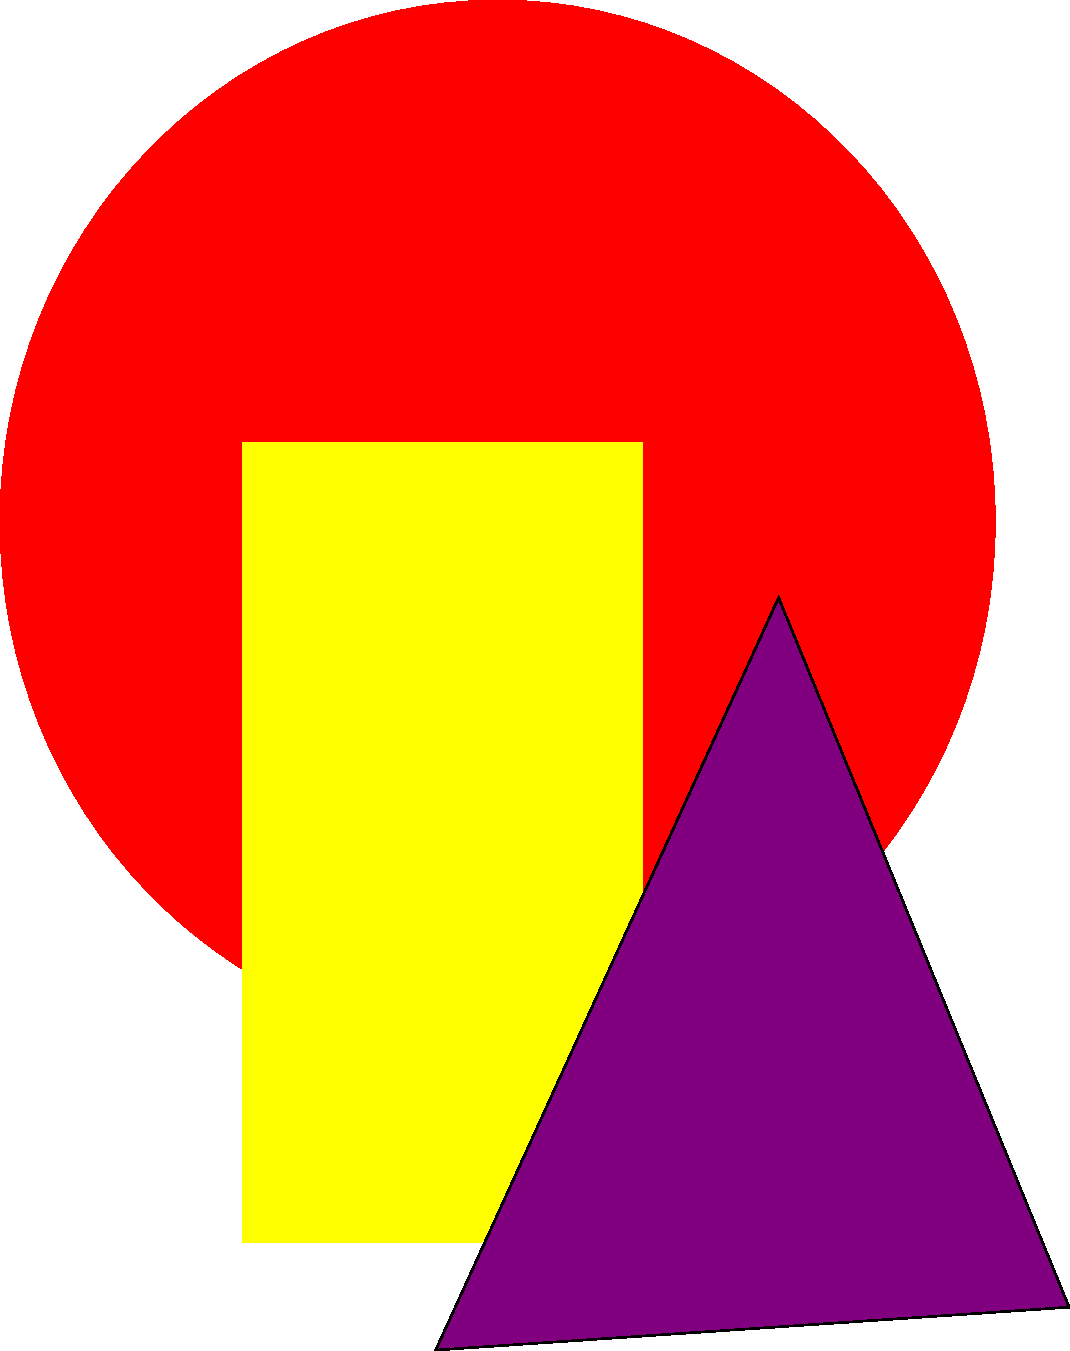
\includegraphics[width=0.8\textwidth,height=6cm]{Imagenes/Arte_abstracto}
%     \caption{Un pie de foto}
%     \label{fig:una_etiqueta}
% \end{figure}


\section{Objetivos y limitaciones}

El objetivo del proyecto es desarrollar un sistema de información en forma de aplicación web que muestra la monitorización en tiempo real de alertas. \newline

Estas alertas pueden ser de dos tipos:
\begin{itemize}
    \item \textbf{Presencias}: son alertas que indican la presencia de un trabajador en una habitación. Estas presencias se muestran en los terminales y pueden ser no identificadas (se pulsa un botón en la pantalla táctil del terminal) o identificadas (el trabajador pasa su tarjeta de identicación por el lector del terminal).
    \item \textbf{Alarmas}: son alertas que se disparan una única vez. Estas son generadas desde los terminales que se encuentran en las habitaciones y pueden ser codificadas por el primer trabajador que se ha identificado en ese terminal.    
\end{itemize}

% Hetereogeneidad de tamaños
Este sistema web servirá para pequeños y grandes escenarios. Es decir será útil para por ejemplo una residencia pequeña en la que el número de clientes, habitaciones y por tanto terminales sea reducido. O el caso contrario en el que se quiera monitorizar las alertas de un hospital de gran tamaño con un alto número de clientes y terminales.

% Explicar concretamente el trabajo a realizar - objetivo más detallado
El trabajo a realizar para llevar a cabo la construcción de la aplicación web consta de dos partes.\\

En primer lugar, implementar un frontend completo desde cero separado de la aplicación actual de Ibernex.\\

En segundo lugar, el desarrollo de un backend que se realiza integrando código en Helpnex aprovechando algunas de las funcionalidades existentes y desarrollando las nuevas funcionalidades necesarias. \newline

La limitación a la hora de realizar el proyecto es que al tener ya una aplicación desarrollada con ciertas tecnologías, se debe realizar el análisis de tecnologías y análisis y diseño del sistema en base a esas condiciones y teniendo en cuenta las necesidades que se podrán ver posteriormente en la sección de requisitos del sistema. 


\section{Herramientas de trabajo}

% TODO: Explicar las tecnoloías que estoy utilizando para cada una de las partes, y las librerías utilizadas.

TODO: ¿Explicar frameworks, tecnologías, entornos de desarrollo, editores de código fuente, git, tortoisegit, github, google met y chat/gmail para comunicación con empresa en remoto?

\section{Esquema general de la memoria del proyecto}

% TODO: Exponer las secciones que pertenecen a la memoria del proyecto para hacer una presentación de lo que se explica en cada una de ellas y no solo con el índice y los títulos.

TODO: redactar una vez clara la estructura final de la memoria








